\chapter{Comparative Analysis of Autonomous Navigation Approaches}%
\label{chap:nav}

\subimport{.}{intro}
\section{Open-Loop and Closed-Loop Navigation}%
\label{sec:nav:principles}

\subsection{Principle of Open-Loop Navigation}%
\label{subsec:nav:openloop-principle}

In open-loop navigation, the complete path is resolved before the drone starts
moving. The planner takes as input a map of the environment, a start position and
a target, then searches for the route that minimises a chosen cost. That cost
need not be distance: flight time, energy consumption or path smoothness are all
used in practice. Once the route has been obtained, the vehicle executes it as
computed. This mode of operation is also known as offline planning, and it
presupposes a static environment~\cite{kumar2025comprehensive}.

Where that assumption holds, it offers a real advantage: the problem is solved
once, on the ground, without the computational constraints of the onboard
hardware.

\subsection{Principle of Closed-Loop Navigation}%
\label{subsec:nav:closedloop-principle}

In closed-loop navigation, the decision is re-derived throughout the flight. The
drone observes its surroundings, updates its internal representation of them, and
selects its next action from that updated state. Online planning rests on the
same principle and is designed for unexpected obstacles and changing
conditions~\cite{kumar2025comprehensive}. Learning-based methods make the
structure explicit: the agent executes an action, the environment returns an
observation and a reward, and both feed back into the following
decision~\cite{chang2023review}.

The benefit is robustness. Fixed waypoints and pre-computed paths adapt poorly to
conditions that evolve and to obstacles that were not anticipated, which raises
the risk of collision~\cite{pore2026uavqr}.



\begin{figure}[htbp]
    \centering
    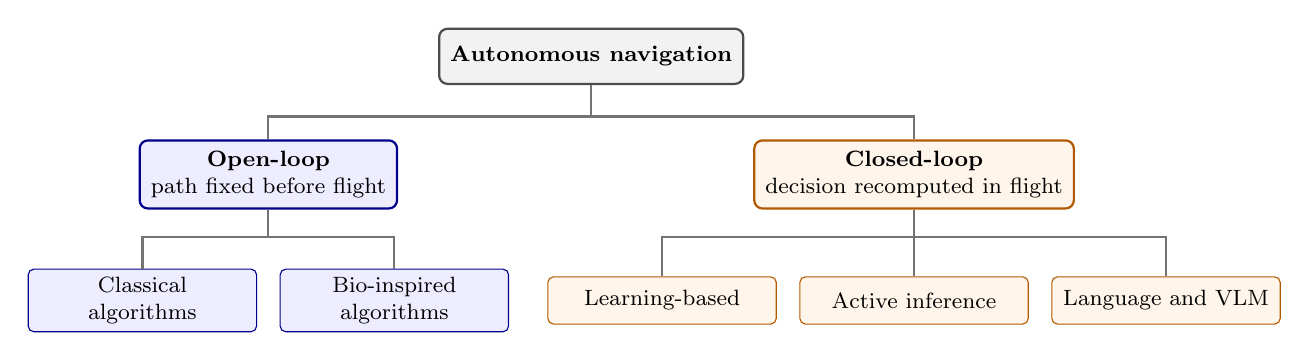
\begin{tikzpicture}[
        font=\small,
        head/.style={rounded corners=3pt, draw, thick, minimum height=0.7cm,
                     align=center, font=\footnotesize\bfseries, inner sep=4pt},
        fam/.style={rounded corners=2pt, draw, minimum height=0.6cm,
                    minimum width=2.9cm, align=center, font=\footnotesize,
                    inner sep=3pt},
        ol/.style={draw=blue!55!black,   fill=blue!7},
        cl/.style={draw=orange!70!black, fill=orange!8},
        line/.style={draw=black!55, thick},
    ]

    \node[head, draw=black!70, fill=black!5] (root) at (0,0)
        {Autonomous navigation};

    \node[head, ol] (ol) at (-4.1,-1.5) {Open-loop\\
        \footnotesize\mdseries path fixed before flight};
    \node[head, cl] (cl) at ( 4.1,-1.5) {Closed-loop\\
        \footnotesize\mdseries decision recomputed in flight};

    \draw[line] (root.south) -- ++(0,-0.4) -| (ol.north);
    \draw[line] (root.south) -- ++(0,-0.4) -| (cl.north);

    \node[fam, ol] (cls) at (-5.7,-3.1) {Classical\\algorithms};
    \node[fam, ol] (bio) at (-2.5,-3.1) {Bio-inspired\\algorithms};

    \draw[line] (ol.south) -- ++(0,-0.35) -| (cls.north);
    \draw[line] (ol.south) -- ++(0,-0.35) -| (bio.north);

    \node[fam, cl] (lrn) at (0.9,-3.1) {Learning-based};
    \node[fam, cl] (aif) at (4.1,-3.1) {Active inference};
    \node[fam, cl] (llm) at (7.3,-3.1) {Language and VLM};

    \draw[line] (cl.south) -- ++(0,-0.35) -| (lrn.north);
    \draw[line] (cl.south) -- ++(0,-0.35) -| (aif.north);
    \draw[line] (cl.south) -- ++(0,-0.35) -| (llm.north);

    \end{tikzpicture}
    \caption{Taxonomy of the navigation methods compared in this chapter.}%
    \label{fig:nav:taxonomy}
\end{figure}

\FloatBarrier
\section{Open-Loop Methods: Classical Algorithms}%
\label{sec:nav:classical}

Classical algorithms come from robotics and operations research, and they form
the first family in the standard taxonomy of trajectory design
methods~\cite{krayani2023goal}. They share one assumption: the workspace is known
before the flight and does not change during the mission. Several of them derive
from dynamic programming, which solves a large decision problem by cutting it
into successive stages.

\subsection{Graph Search: Dijkstra and A*}%
\label{subsec:nav:graphsearch}

The workspace is represented as a graph, where each node is a position and each
edge carries a cost. Finding a path becomes finding the cheapest chain of edges
between two nodes.

Dijkstra explores the graph outwards from the start, like a circle that keeps
growing, and stops when it reaches the goal. Every direction is explored, so the
path is always the shortest one, but many nodes are visited for
nothing~\cite{chang2023review}.

A* adds an estimate of the distance remaining to the goal and expands the node
whose total cost, travelled plus estimated, is the lowest. The search becomes
directed and reaches the goal after far fewer nodes. Its result depends on the
quality of that estimate, and the vehicle moves only between neighbouring nodes,
which produces a route with sharp turns~\cite{kumar2025comprehensive}.

\subsection{Incremental Replanning: D* and Its Variants}%
\label{subsec:nav:dstar}

D* addresses what happens when the map turns out to be wrong. Instead of
searching again from the start, it keeps the costs already computed and updates
only the nodes whose cost has changed~\cite{krayani2023goal}. If an obstacle
appears in one aisle, the rest of the path is reused as it is.

The method needs a complete initial path to repair, and it gives no guarantee on
the result when the environment keeps
changing~\cite{kumar2025comprehensive, krayani2023goal}. It therefore sits on the
border of the two families: the path is computed in advance, but it is revised
during the flight.

\subsection{Mixed-Integer Linear Programming}%
\label{subsec:nav:milp}

The methods that follow do not search a graph. They state the mission as an
optimisation problem and hand it to a solver.

Linear programming minimises a linear function under linear constraints.
Mixed-integer linear programming extends this to problems that mix continuous
variables, such as a position, with discrete ones, such as the decision to visit
a point or not~\cite{kumar2025comprehensive}.

For a drone, the flight is discretised into time steps. Each step becomes a set
of variables describing the state of the vehicle, the constraints encode the
obstacles, and the solver returns a complete trajectory before the mission
starts. The formulation is offline by construction and does not scale to long
trajectories~\cite{krayani2023goal}.

\subsection{Coverage and Routing Formulations}%
\label{subsec:nav:tsp}

These formulations apply when the mission is to visit several places rather than
reach one goal. In the travelling salesman problem, the drone passes through a
fixed set of points, visits each one exactly once, and returns to its starting
position before the battery runs out. The problem is NP-hard, so practice relies
on local-search heuristics such as 2-OPT~\cite{krayani2023goal}.

Its profit variant gives each point a reward, and the objective becomes a
compromise between distance travelled and reward collected. The limitation is
structural: the tour is computed once, so a new target appearing during the
flight forces the whole route to be recomputed~\cite{krayani2023goal}.

\subsection{Coverage Path Planning}%
\label{subsec:nav:cpp}

Coverage path planning applies when the mission is not to reach a position but to
pass over every part of a known area. The workspace is first decomposed into
regions that the vehicle can sweep without interruption, then an order is chosen
between these regions, and finally a motion pattern fills each one. In a
structured space such as a warehouse, the decomposition is given by the layout
itself: each aisle is a region, and the pattern reduces to travelling along it
while facing the racks.

The route is therefore complete before take-off, and it covers the whole area
whatever it contains. What separates the existing systems is the criterion they
optimise inside that route. Some weight the aisles by the density of codes
detected, so that flight time is spent where there is something to
read~\cite{kalinov2020warevision}. Others extend the problem to a heterogeneous
team and solve the order of every operation in advance, including the moments
when the ground robots carry the drones and deploy the
beacons~\cite{guinand2021uavugv}. A third group keeps a safety margin along each
aisle and revises the route over a short horizon when new risk information
arrives, without claiming full real-time avoidance of moving
obstacles~\cite{pore2026uavqr}.

The limitation is the same in every case. The sweep is computed from a layout
that must be known, and a region discovered during the flight has no place in a
route that was already closed.

\section{Open-Loop Methods: Biologically Inspired Algorithms}%
\label{sec:nav:metaheuristics}

The previous section ended on a difficulty: routing formulations are NP-hard, so
the exact optimum becomes unreachable as soon as the number of targets grows.
Evolutionary optimisation is the usual answer, and it has proved effective at
reducing the total distance travelled in real cases~\cite{krayani2023goal}.

These algorithms all work the same way. A population of candidate paths is
generated, each one is scored, and the population is improved over many
iterations until the result stops getting better. They do not compute the best
solution but a good one, and they give no guarantee of
optimality~\cite{kumar2025comprehensive}.

\subsection{Genetic Algorithm}%
\label{subsec:nav:ga}

The genetic algorithm imitates natural selection. The best paths of the current
population are selected, then combined by crossover, which builds a new path from
two existing ones, and altered by mutation, which changes a part of a path at
random. Over the generations, the population drifts towards better
routes~\cite{kumar2025comprehensive}.

Its weakness is speed. Convergence is slow, which makes it unsuitable for any
planning problem that needs a fast answer~\cite{krayani2023goal}.

\subsection{Particle Swarm Optimization}%
\label{subsec:nav:pso}

Particle swarm optimisation imitates a flock of birds. Each particle is a
candidate path, and it moves through the search space under two influences: the
best position it has found itself, and the best position found by the whole
swarm. The swarm therefore concentrates around the promising regions.

It is fast and good at refining a solution locally, which is why it is often
paired with a genetic algorithm handling the global search~\cite{krayani2023goal}.
Its weakness is the other side of that strength: the swarm converges too early
and settles on a solution that is not the best
one~\cite{kumar2025comprehensive}.

\subsection{Ant Colony Optimization}%
\label{subsec:nav:aco}

Ant colony optimisation imitates how ants find the shortest route to a food
source. Artificial ants build candidate paths and leave a pheromone trail on the
route they used. A short route is travelled more often, so it accumulates more
pheromone and attracts more ants, while the trails on the other routes evaporate.
The colony converges on a good tour without any central
decision~\cite{kumar2025comprehensive}.

Its weakness is cost. The iterations are slow and the method needs a large amount
of data before it converges~\cite{krayani2023goal}.





\section{Limits of Open-Loop Methods}%
\label{sec:nav:openloop-limits}

The two families presented above differ in the way they search for a solution,
but not in what they assume before the search starts. Four limits follow from
that shared assumption.

\begin{itemize}[itemsep=0.5em]
    \item \textbf{The environment must be known in advance}: Planning begins with
          a model of the environment in which the obstacles are already
          identified. Whatever form this model takes, a graph, a grid or a list
          of targets with their costs, it has to exist before the
          flight~\cite{kumar2025comprehensive}.
    \item \textbf{The plan does not adapt during the mission}: Offline planning
          assumes a static environment, so a route computed on the ground stays
          valid only as long as nothing changes. Pre-computed paths handle poorly
          the obstacles that were not anticipated, which raises the risk of
          collision~\cite{pore2026uavqr}.
    \item \textbf{Replanning is expensive}: When something does change, most of
          these methods start again from the beginning. D* is the exception,
          since it repairs only the affected part of the path, but even D* needs
          a complete initial path to repair~\cite{krayani2023goal}.
    \item \textbf{Coordination between drones is decided before take-off}: In a
          multi-\gls{abb:uav} mission, the targets are assigned and the workload
          balanced as part of the plan computed on the ground. Allocation able to
          adapt in real time is presented in the literature as a future
          direction, not as current practice~\cite{kumar2025comprehensive}.
\end{itemize}
\section{Closed-Loop Methods: Learning-Based Approaches}%
\label{sec:nav:learning}

Learning-based methods form the third family in the standard
taxonomy~\cite{krayani2023goal}. They abandon the idea of computing a route
altogether. Instead of planning, the agent tries an action, observes what happens
and adjusts its behaviour, over and over, until it knows what to do in each
situation. What it ends up with is not a path but a \emph{policy}: a rule that
maps any situation to an action.

The loop has four elements. The agent performs an action, the environment moves
to a new state and returns a reward, and both feed back into the next
decision~\cite{chang2023review}. The reward is the only signal the agent
receives, and its entire behaviour is shaped by it.

The problem is written as a Markov decision process. When the drone cannot
observe the true state of the world, as happens indoors with noise and occlusion,
it becomes a partially observable one: the agent no longer knows where it is and
maintains a \emph{belief}, a probability distribution over the possible states,
which it updates after every observation~\cite{sandino2020autonomous}. In both
cases the objective is the same, namely to find the policy that maximises the sum
of future rewards, each weighted by a discount factor that reduces the importance
of what lies far ahead.

\subsection{Reinforcement Learning Methods}%
\label{subsec:nav:rl}

\textbf{Q-learning.} Rather than learning a policy directly, the agent learns a
value $Q(s,a)$ for every state--action pair, which estimates the total return
expected from taking action $a$ in state $s$~\cite{chang2023review}. These values
are kept in a table, initialised arbitrarily, and corrected at every step:

\begin{equation}
    Q(s_t, a_t) \leftarrow Q(s_t, a_t) + \alpha \Bigl[ r_t
    + \gamma \max_{a'} Q(s_{t+1}, a') - Q(s_t, a_t) \Bigr]
    \label{eq:nav:qlearning}
\end{equation}

The bracket is the correction. The agent expected $Q(s_t, a_t)$; what it actually
obtained is the immediate reward $r_t$ plus the best value available from the
state it landed in, $\max_{a'} Q(s_{t+1}, a')$. The difference between the two is
the error, and the learning rate $\alpha$ decides what fraction of it is applied.
The discount factor $\gamma$ reduces the weight of what lies further ahead. Once
the table has converged, acting consists in reading the line of the current state
and taking the action with the highest value.

Learning is slow, because each step corrects a single entry of the table, and the
algorithm cannot explain why an action was wrong~\cite{krayani2022novel}.

\textbf{Deep Q-networks.} A table becomes impossible when the state is an image
or a map, since there are far too many states to enumerate. The table is
therefore replaced by a neural network that takes the state as input and returns
the value of each action. The network is trained on past transitions, stored and
replayed in batches so that successive samples are no longer
correlated~\cite{ding2024external}. The method still needs a large number of
samples, and the action set must stay discrete, since the network returns one
value per action.

\textbf{Policy-gradient and actor-critic methods.} These learn the policy itself
instead of the values, which lifts the discrete-action restriction and allows a
continuous output such as a velocity or a heading. Two networks are used: the
\emph{actor} produces the action, and the \emph{critic} estimates how good it
was. The critic's judgement is what adjusts the actor. Training is unstable,
because both networks change at once, so a delayed copy of each is kept as a
fixed reference~\cite{ding2024external}.

\textbf{Multi-agent reinforcement learning.} The framework is extended to several
drones. Each keeps its own actor-critic network and decides from its own local
state, but the reward measures the performance of the whole team, which is what
pushes the agents to cooperate. No central coordinator is needed, so the
communication overhead stays low~\cite{ding2024external}.

\subsection{Online POMDP Solvers}%
\label{subsec:nav:pomdp-solvers}

These solvers use the same formalism but learn nothing at all. There is no
training phase and no policy: at every step, the agent simulates what would
happen after each candidate action, starting from its current belief, and takes
the action whose simulated outcome is best. The whole computation is repeated at
the next step, from the updated belief.

The Adaptive Belief Tree follows this principle and has been used for navigation
in cluttered, \gls{abb:gps}-denied environments, where noise and occlusion
prevent the drone from observing the true state~\cite{sandino2020autonomous}.

Removing the training phase moves the cost to the flight itself. Running these
simulations together with object detection on the onboard computer of a small
drone is an open challenge~\cite{sandino2020autonomous}.

\subsection{Limits of Learning-Based Approaches}%
\label{subsec:nav:learning-limits}

\begin{itemize}[itemsep=0.5em]
    \item \textbf{Training cost}: A trained network answers quickly, but training
          itself requires a large number of samples and considerable
          time~\cite{krayani2026bayesian}.
    \item \textbf{Poor generalisation}: These methods adapt badly to situations
          absent from their training set, and adapting them means retraining
          them~\cite{krayani2023goal, krayani2026bayesian}.
    \item \textbf{Onboard computation}: Decision and perception must run together
          on limited hardware, which remains an open
          difficulty~\cite{sandino2020autonomous}.
    \item \textbf{Reward design}: The behaviour of the agent depends entirely on
          a reward function written by hand, whose weights must be tuned for each
          mission~\cite{ding2024external}.
\end{itemize}    
\section{Closed-Loop Methods: Active Inference}%
\label{sec:nav:activeinf}

Active inference comes from neuroscience. The idea is that the brain does not
passively receive information: it constantly predicts what it is about to
perceive and reacts when reality does not match the prediction. This behaviour is
described by a single rule, the minimisation of what is called free
energy~\cite{ding2024external}, and robotics later reused that rule to control
machines~\cite{ji2023delay}.

The difference with the previous section lies in the objective. A reinforcement
learning agent depends entirely on the reward the environment returns. An active
inference agent receives no reward: it carries an internal model of the world, an
expectation of what it should observe, and its only goal is to reduce the gap
between that expectation and what its sensors report.

\subsection{The Free Energy Principle}%
\label{subsec:nav:fep}

When a gap appears between the model and reality, the agent has two ways of
reducing it. It can update its beliefs to match the observations, or it can act
on the world so that the observations match the model again. The two mechanisms
form a loop: what the agent believes determines what it does, and what it does
changes what it observes~\cite{ji2024integration}.

The quantity to minimise is \emph{surprise}, meaning how unexpected the current
observation is. It cannot be computed, because that would require considering
every possible cause of an observation. The framework therefore replaces it by
two quantities that can be computed: one for understanding the present, one for
choosing the future~\cite{ji2024integration}.

\subsection{Variational Free Energy}%
\label{subsec:nav:vfe}

Variational free energy answers the question \emph{where am I and what is
happening around me?}. The drone cannot know the true state of the world, only
what its sensors show, so it maintains an approximate answer and brings it as
close as possible to the truth. Free energy measures the distance that
remains~\cite{ji2024integration}.

The same quantity serves twice. Minimising it by changing beliefs is perception;
minimising it by changing actions is control. In both cases the model ends up
explaining the observations better. In practice it plays the role of a loss
function: a number the system pushes down~\cite{ji2024integration}.

\subsection{Expected Free Energy}%
\label{subsec:nav:efe}

Variational free energy only looks at the present, so it says nothing about the
next action~\cite{ding2024external}. Expected free energy fills that gap: for
each candidate action, the agent imagines what would follow, computes the free
energy that action would produce, and keeps the lowest.

What makes this quantity interesting is that it splits into two terms. The first
is high when an action would teach the agent something new, which pushes towards
exploration. The second is high when an action brings the agent closer to the
situation it wants, which pushes towards the goal~\cite{fang2024resource}. A
drone minimising expected free energy therefore gathers information and pursues
its objective at the same time~\cite{wang2026bridging}.

This is the main attraction of the framework. In reinforcement learning,
exploration has to be added by hand through a bonus in the reward. Here it comes
out of the same expression as the goal.


\subsection{Limits of Active Inference}%
\label{subsec:nav:aif-limits}

\begin{itemize}[itemsep=0.5em]
    \item \textbf{The model of the world must be built first}: Nothing can be
          inferred without an internal model. In the trajectory design work, it
          is learned before the mission from examples produced by an expert
          optimiser, so the difficulty is moved rather than
          removed~\cite{krayani2023goal, krayani2026bayesian}.
    \item \textbf{Exact computation is impossible}: The framework always works
          with approximations, and in practice assumes that the distributions are
          Gaussian~\cite{ji2024integration}.
    \item \textbf{Scaling up requires neural networks}: Which brings back part of
          the training cost that active inference was supposed to
          avoid~\cite{ding2024external}.
    \item \textbf{Multi-agent use is still rare}: The framework works well for a
          single agent, but existing multi-drone frameworks are centralised,
          which makes them hard to place inside a modular
          architecture~\cite{wang2026bridging}.
\end{itemize}

The next section presents a more recent family of closed-loop methods, where the
internal model of the environment is replaced by a pre-trained language or
vision-language model.
\section{Closed-Loop Methods: Language and Vision-Language Models}%
\label{sec:nav:genai}

The two previous families both need a model of the world and both have to obtain
it: reinforcement learning builds it through a large number of trials, active
inference receives it from the engineer. The family presented here takes a
different route, because the model already exists. It is a network trained on
very large amounts of image and text data, and it carries a general knowledge of
the world that can be reused without any training specific to the task. This
property is what the literature calls zero-shot~\cite{radford2021learning}.

What changes from one method to another is the role this model plays inside the
decision loop. Three roles can be distinguished, each giving the robot more
autonomy than the previous one.

\subsection{The Model as an Instruction Interpreter}%
\label{subsec:nav:genai-interface}

In the first role, the model translates what a human asked for. The user
describes the task in ordinary language, and the model produces a plan written in
a command set defined for the robot. Everything depends on the prompt, which
lists the available functions, shows a few worked examples, and states the rules
the answer must follow~\cite{vemprala2023chatgpt}. TypeFly applies this to a
drone, adding the current state of the scene to that
prompt~\cite{chen2024typefly}.

The difficulty is that the model knows the world but not the machine it controls.
It can propose an action that makes sense in principle and is impossible in
practice. SayCan answers this by combining two scores: how useful the language
model judges an action to be, and how likely a previously learned value function
judges it to succeed from the current state. The product of the two selects the
action, and the language model itself is never
retrained~\cite{ahn2022saycan}.

In this role, the robot executes rather than decides. Something still has to tell
it what to do.

\subsection{The Model as a Semantic Sensor}%
\label{subsec:nav:genai-vlm}

In the second role, the model interprets what the camera sees. A language model
does not see, so the scene must first be described to it, and there are two ways
of doing so.

The first is a discrete description. A light detector lists the objects visible
in the image with their bounding boxes, and this list enters the prompt. TypeFly
uses YOLOv8 this way: the object type feeds the reasoning, the bounding box
locates the target~\cite{chen2024typefly}. The vocabulary is closed, however, so
the robot only reasons about categories the detector was trained on, and every
visual cue has to pass through the detector before it can be
used~\cite{yokoyama2024vlfm}.

The second avoids this conversion. CLIP trains an image encoder and a text
encoder together on a single objective: given a batch of images and a batch of
texts, predict which pairs go together. Both modalities then live in the same
space, so comparing an image with a description reduces to a dot product between
two vectors. A class no longer has to be a label seen during training; it can be
any sentence, which is how zero-shot recognition becomes
possible~\cite{radford2021learning}.

\subsection{The Model as an Exploration Guide}%
\label{subsec:nav:genai-navigation}

In the third role, the model orients the decision itself. There is no human
instruction and no map: the robot is given the name of a target and must explore
an environment it has never seen in order to find it.

The geometric basis of this behaviour is frontier-based exploration. A frontier
is a boundary between the explored region of the map and the region still
unknown, on a map the agent builds as it moves, and exploring means going to
these boundaries. Classical methods select the frontier expected to reveal the
largest amount of new information~\cite{yokoyama2024vlfm}.

Semantic guidance replaces that criterion: instead of asking which frontier
reveals the most, the robot asks which one most likely leads to the target. L3MVN
describes in text the objects around each frontier and asks a language model
which description best matches the target~\cite{yu2023l3mvn}. VLFM removes the
text step: a vision-language model computes a similarity between the current
image and a prompt containing the target, and this score is projected onto a
top-down value map, whose highest frontier becomes the next
waypoint~\cite{yokoyama2024vlfm}.

Both report strong results. VLFM reaches state-of-the-art performance on three
photorealistic datasets without task-specific training and without a pre-built
map, and was deployed on a Boston Dynamics Spot robot in an office
building~\cite{yokoyama2024vlfm}. L3MVN outperforms map-based methods in success
rate and generalisation, and was also validated on a real
robot~\cite{yu2023l3mvn}.

In this role, the pre-trained model neither executes nor describes. It selects
where the robot goes.

\subsection{Limits of Language-Based Approaches}%
\label{subsec:nav:genai-limits}

\begin{itemize}[itemsep=0.5em]
    \item \textbf{Computation and latency}: These models require a large amount
          of computing power, which usually means running them on a remote
          server, and detailed prompts are more expensive than short
          ones~\cite{chen2024typefly}.
    \item \textbf{Reliability of the output}: Nothing guarantees that a proposed
          action can be executed, which is why a grounding mechanism is
          required~\cite{ahn2022saycan}.
    \item \textbf{Representation tied to a single target}: The value map built by
          VLFM holds only the information relevant to the current target, so it
          cannot be reused for another one~\cite{yokoyama2024vlfm}.
    \item \textbf{Validation}: Results come mainly from indoor household
          benchmarks, on ground platforms, and VLFM further assumes that the
          target is visible from the default camera height and does not handle
          changes of floor~\cite{yokoyama2024vlfm, yu2023l3mvn}.
\end{itemize}
\section{Comparative Synthesis and Identified Gaps}%
\label{sec:nav:synthesis}

This chapter has presented five families of navigation methods, one after the
other. To compare the individual works on a common basis,
\Cref{tab:nav:synthesis} brings them together. The columns cover what the method
needs to know before the mission, when it chooses its target, what criterion
guides that choice, how several agents share the work, whether the method was
tested on a robot, and how it was evaluated.

\begin{sidewaystable}
    \centering
    \caption{Comparative analysis of decision-making approaches.}%
    \label{tab:nav:synthesis}
    \footnotesize
    \setlength{\tabcolsep}{2pt}
    \begin{tabular}{@{}>{\raggedright\arraybackslash}p{2.3cm}
            >{\raggedright\arraybackslash}p{2.7cm}
            >{\raggedright\arraybackslash}p{2.1cm}
            >{\raggedright\arraybackslash}p{1.4cm}
            >{\raggedright\arraybackslash}p{2.5cm}
            >{\raggedright\arraybackslash}p{1.8cm}
            >{\raggedright\arraybackslash}p{2.3cm}
            >{\raggedright\arraybackslash}p{2.1cm}
            >{\raggedright\arraybackslash}p{2.9cm}
            >{\raggedright\arraybackslash}p{2.1cm}@{}}
        \toprule
        \textbf{Work} & \textbf{Decision family} & \textbf{Known before the
        mission} & \textbf{Target chosen} & \textbf{What drives the choice} &
        \textbf{Multi-agent} & \textbf{Work sharing} & \textbf{Robotic
        platform} & \textbf{Metrics used} & \textbf{Validation} \\
        \midrule
        \textcite{kalinov2020warevision} & Classical                                    & Rack layout           & Before flight & Detection density                               & No                                                  & ---                          & Yes, drone + \glsxtrshort{abb:ugv} & Inspection time, recognition rate       & Laboratory                \\
        \addlinespace
        \textcite{guinand2021uavugv}     & Classical, offline optimisation              & Full layout           & Before flight & Makespan                                        & Yes, \glsxtrshort{abb:uav}s + \glsxtrshort{abb:ugv}s & Central schedule             & Yes, drones                        & Makespan                                & Model only                \\
        \addlinespace
        \textcite{pore2026uavqr}         & Classical + short replanning                 & Aisle layout          & Before flight & Path length, safety                             & Yes, 2 \glsxtrshort{abb:uav}s                       & Fixed split, cloud filtering & Yes, drones                        & Decoding rate, mission time, duplicates & Simulation + real testbed \\
        \addlinespace
        \textcite{chandran2024network}   & Coverage, decentralised                      & Area to cover         & Before flight & Coverage time                                   & Yes, swarm                                          & Leader broadcasts waypoints  & Yes, drones                        & Mission time, packet delivery, delay    & Simulation                \\
        \addlinespace
        \textcite{sandino2020autonomous} & Online \glsxtrshort{abb:pomdp}               & Nothing               & Online        & Discounted reward                               & No                                                  & ---                          & Yes, drone                         & Success rate, flight time               & Simulation                \\
        \addlinespace
        \textcite{krayani2023goal}       & Active inference                             & Generative model      & Online        & Expected free energy                            & No                                                  & ---                          & No, wireless network               & Convergence speed, collected profit     & Simulation                \\
        \addlinespace
        \textcite{ding2024external}      & Deep \glsxtrshort{abb:rl} + active inference & Nothing               & Online        & Reward, then free energy                        & Yes                                                 & Global reward                & No, wireless network               & Sum-rate, convergence                   & Simulation                \\
        \addlinespace
        \textcite{wang2026bridging}      & Active inference + behaviour trees           & Behaviour tree, model & Online        & Expected free energy                            & Yes                                                 & Node-level inference         & Yes, drones                        & Tree complexity, task success           & Simulation                \\
        \addlinespace
        \textcite{ahn2022saycan}         & \glsxtrshort{abb:llm} + affordances          & Skill library         & Online        & \glsxtrshort{abb:llm} score $\times$ feasibility & No                                                  & ---                          & Yes, ground robot                  & Plan success, execution success         & Real robot                \\
        \addlinespace
        \textcite{chen2024typefly}       & \glsxtrshort{abb:llm} + detector             & Command set           & Online        & \glsxtrshort{abb:llm} plan over object list      & No                                                  & ---                          & Yes, drone                         & Task success, latency                   & Real drone                \\
        \addlinespace
        \textcite{yu2023l3mvn}           & \glsxtrshort{abb:llm} + frontiers            & Nothing               & Online        & \glsxtrshort{abb:llm} score over frontier text   & No                                                  & ---                          & Yes, ground robot                  & Success rate, SPL                       & Simulation + real         \\
        \addlinespace
        \textcite{yokoyama2024vlfm}      & \glsxtrshort{abb:vlm} + frontiers            & Nothing               & Online        & Image--text similarity                          & No                                                  & ---                          & Yes, ground robot                  & Success rate, SPL                       & Simulation + real         \\
        \bottomrule
    \end{tabular}

    \vspace{0.6em}
    {\footnotesize SPL: success weighted by normalised inverse path length.}
\end{sidewaystable}

\FloatBarrier

\paragraph{No system inspects a warehouse it does not know.} Inventory systems
receive the layout of the aisles before take-off and follow a route computed on
the ground. The systems that explore without a map do not perform inventory, and
none of them flies: they are ground robots looking for one designated object in a
house or an office, and they stop as soon as they find
it~\cite{yokoyama2024vlfm, yu2023l3mvn}. The only drone that reasons about the
content of the scene executes an instruction given by a human rather than
deciding for itself~\cite{chen2024typefly}.

\paragraph{No system redistributes the work when a drone stops flying.} The
division is decided on the ground, through a central
schedule~\cite{guinand2021uavugv}, a fixed split between two
drones~\cite{pore2026uavqr}, or a leader that sends the waypoints to the
group~\cite{chandran2024network}. Once the vehicles are in the air, nothing
changes hands. If one of them stops flying, the share it was holding is left with
no owner.

\paragraph{No system allocates targets from what the drones discover.}
Multi-drone systems avoid duplicated readings because the division was fixed
before take-off, and none of them reassigns a target that appears during the
mission. The literature states the same thing: allocation able to adapt in real
time is described as a future direction rather than as current
practice~\cite{kumar2025comprehensive}.

\paragraph{No system knows when the inventory is complete.} Systems that follow a
computed route stop at the end of that route. Ground robots that explore stop as
soon as they have found the object they were looking for, since finding it is
their mission~\cite{yokoyama2024vlfm}. None of them estimates what remains to be
read in order to decide by itself when to stop.

\paragraph{No system decides from what it sees and cooperates at the same time.}
Two separate worlds coexist. On one side, ground robots choose their direction
from the content of the scene, but they work alone and look for a single object
in a house or an office~\cite{yokoyama2024vlfm, yu2023l3mvn}. On the other,
drones perform inventory as a team, but they decide from a time, a distance or a
score, and they follow a route computed before take-off. No work carries the
reasoning about the scene from the first world into the second.

\bigskip

Taken together, these gaps describe one missing system. There is no system in
which several drones explore an unknown warehouse, produce their targets from
what they observe, and share those targets between them while the mission is
running.

\section{Chapter Conclusion}%
\label{sec:nav:conclusion}

This chapter studied the layer that the previous one identified as the real
difficulty: how a drone decides where to go next. The comparison used one
criterion, the moment when the path is decided, which separates the methods that
compute the whole route before take-off from those that choose the next move
during the flight.

The open-loop methods came first, in their classical and biologically inspired
forms. They search in different ways but need the same thing, a description of
the workspace before the flight, and when something changes they replan from the
beginning. The closed-loop methods came next, in three families. Learning-based
methods handle the unknown but generalise poorly outside their training
conditions. Active inference removes the external reward but needs a model of the
world that must be built first. Language and vision-language models are the only
family that explores an unknown space without a map and without specific
training, by choosing where to go from the meaning of what the camera sees.

Comparing the individual works then revealed five gaps. No system inspects a
warehouse it does not know. No system redistributes the work when a drone stops
flying, nor allocates targets from what the drones discover. No system knows when
the inventory is complete. And no system decides from what it sees while
cooperating with others, since the two capabilities belong to two separate bodies
of work.

These gaps define the space in which the rest of this work is placed. The next
part presents the system built to fill it, its architecture, and the choices made
during its implementation.
